\lstset{style=sqlstyle}

%CHAPTER
\chapter{Ověření efektivního vytěžování}
K ověření efektivního vytěžování bylo připraveno několik scénářů jak pro SQL, tak i pro Mongo s využitím vyhledávače Elasticsearch. Z výsledků scénářů můžeme poté usoudit, jak moc efektivní vytěžování je vzhledem k technickým parametrům stroje a použitým technologiím.

\subsubsection{Testovací stroj - technické parametry}
Testovací stroj, který byl použit pro kontrolu efektivity vytěžování, má tyto technické parametry:
\begin{itemize}
\item \textbf{Procesor} - Intel(R) Core(TM) i5-6300HQ CPU @ 2.30GHz
\item \textbf{RAM} - 16 GB
\item \textbf{Disk} - SSD 512 GB
\item \textbf{Grafická karta 1} - Intel(R) HD Graphics 539
\item \textbf{Grafická karta 2} - NVIDIA GeForce GTX 960M
\item \textbf{Operační systém} - Linux Manjaro 21.2.6

\end{itemize}

\section{MongoDB + Elasticsearch}
Pro MongoDB a Elasticsearch byly připraveny tři jednoduché scénáře, u kterých byla testována hlavně rychlost odpovědi na zadaný dotaz. Pro dotazování byly použity dotazy typu \textit{query\_string}, které využívají syntaxi k analýze a rozdělení řetězce dotazu na základě operátorů, jako je například AND nebo NOT \cite{elastic_query}.

\newpage
\subsection{Scénář č.1}
\textbf{Textový popis}: Najdi dokumenty, které obsahují jméno \textbf{Porras Vila FCO. Javier} nebo \textbf{Porras Vila F. Javier}.
\newline
\textbf{Dotaz}: 
\begin{lstlisting}[label = {lst:elements_a}]
{
  "query": 
   {
    "query_string": 
      {
       "query": " "PORRAS" AND "VILA" AND "JAVIER" AND ("FCO." OR "F.") "
      }
   }
}
\end{lstlisting}
\textbf{Rychlost vykonání dotazu}: \textpm 0,15 sekund
\newline
\textbf{Výsledek dotazu}: Dotaz vrátil celkem 129 dokumentů obsahující zadané jméno. Ukázku výskytu jména v nalezeném dokumentu lze vidět na obrázku č. \ref{fig:scenar_1_mongo}.
\begin{figure}[H]
\centering
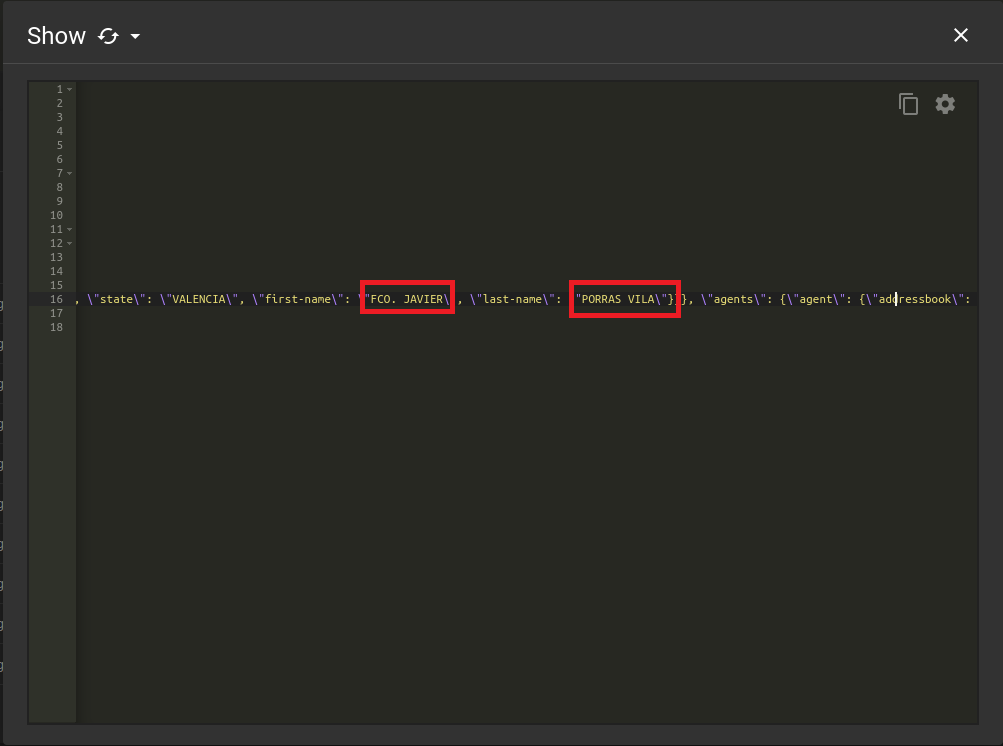
\includegraphics[width=14cm]{img/scenare/scenar_1_mongo}
\caption{Ukázka výsledku dotazu pro scénář č.1}
\label{fig:scenar_1_mongo}
\end{figure}

\newpage
\subsection{Scénář č.2}
\textbf{Textový popis}: Vyhledej dokumenty, které jsou z \textbf{Velké Británie} a klasifikační řetězec je \textbf{E02D}.
\newline
\textbf{Dotaz}: 
\begin{lstlisting}[label = {lst:elements_a}]
{
   "query": 
   {
      "query_string": 
      {
         "query": "\"country: GB\" AND \"subclass: E02D\" "
      }
   }
}
\end{lstlisting}
\textbf{Rychlost vykonání dotazu}: \textpm 0,1 sekund
\newline
\textbf{Výsledek dotazu}: Celkem bylo nalezeno 257 dokumentů (v případě Velké Británie žurnálů). Ukázku výskytu klasifikačního řetězce lze vidět na obrázku č. \ref{fig:scenar_2_mongo}.
\begin{figure}[H]
\centering
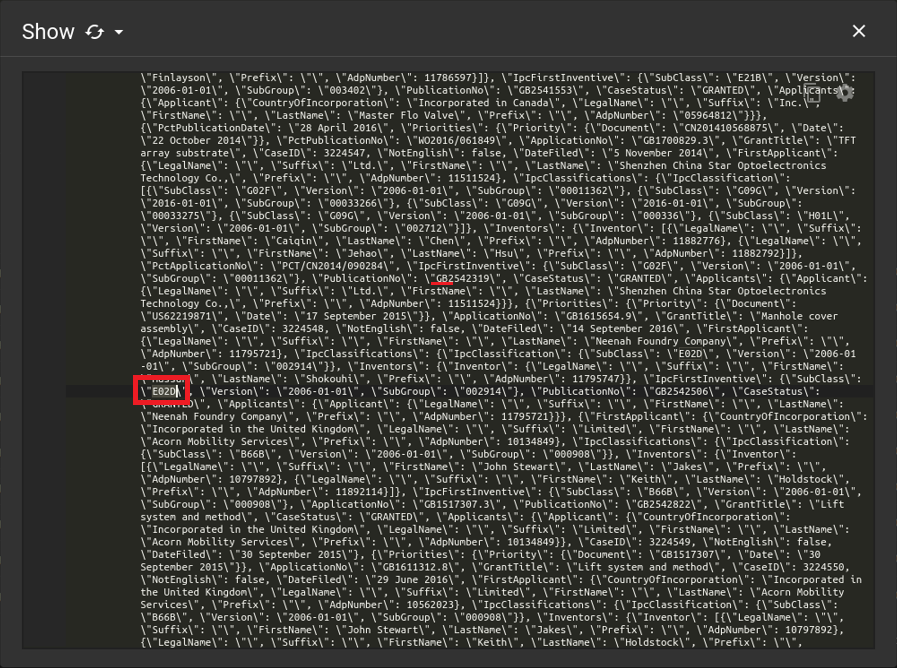
\includegraphics[width=14cm]{img/scenare/scenar_2_mongo}
\caption{Ukázka výsledku dotazu pro scénář č.2}
\label{fig:scenar_2_mongo}
\end{figure}

\newpage
\subsection{Scénář č.3}
\textbf{Textový popis}: Vyhledej dokumenty, který obsahují řetězce s prefixem \textbf{bio} (s posílením 4) a řetězec \textbf{qualcomm} (s posílením 2), nebo obsahují řetězce podobné řetězci \textbf{SANOFI} (neboli \textit{fuzziness}).
\newline
\textbf{Dotaz}: 
\begin{lstlisting}[label = {lst:elements_a}]
{
   "query": 
   {
      "query_string": 
      {
         "query": "((bio*)^4 AND \"qualcomm\"^2) OR (SANOFI~)",
         "analyze_wildcard": true
      }
   }
}
\end{lstlisting}
\textbf{Rychlost vykonání dotazu}: \textpm 3 sekundy
\newline
\textbf{Výsledek dotazu}: Celkem bylo nalezeno 9080 dokumentů, které odpovídají zadanému dotazu. Ukázku výsledku lze vidět na obrázku č. \ref{fig:scenar_3_mongo}.
\begin{figure}[H]
\centering
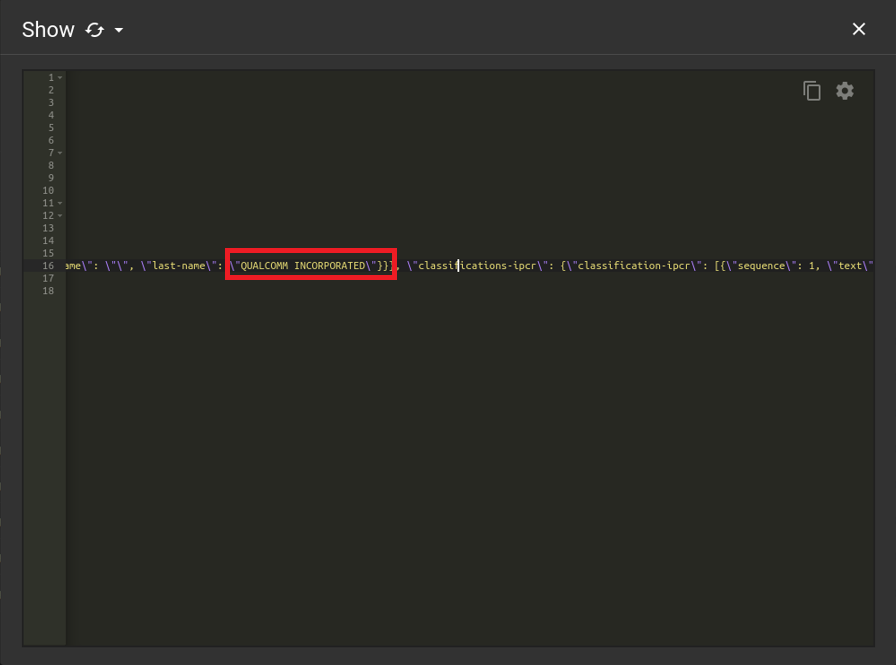
\includegraphics[width=14cm]{img/scenare/scenar_3_mongo}
\caption{Ukázka výsledku dotazu pro scénář č.3}
\label{fig:scenar_3_mongo}
\end{figure}

\newpage
\section{MySQL} \label{sec:efektivni_vytezovani_sql}
Pro MySQL bylo připraveno devět scénářů, které testují všechny vytvořené tabulky v databázi. Každý scénář obsahuje textový popis, název pohledu, pod kterým je scénář uložen, SQL příkaz, rychlost vykonání příkazu a ukázku výsledků. Každý scénář odpovídá jednomu pohledu v databázi.

\subsection{Scénář č.1}
\textbf{Textový popis}: Deset nejčastěji patentujících institucí / autorů v Izraeli v~roce 2015.
\newline
\textbf{Název pohledu}: ten\_IL\_institutes\_2015
\newline
\textbf{SQL}: 
\begin{lstlisting}[label = {lst:elements_a}]
select count(*), count(*) * 100.0 / ((select count(*) from inventors left outer join patents on inventors.id_patent = patents.id where YEAR(patents.patent_date) = 2015 and patents.patent_id like '%IL%') * 1.0) as percentage, inventors.inventor from inventors left outer join patents on inventors.id_patent = patents.id where YEAR(patents.patent_date) = 2015 and patents.patent_id like '%IL%' group by inventors.inventor order by count(*) desc, percentage desc LIMIT 10;
\end{lstlisting}
\textbf{Rychlost vykonání dotazu}:  \textpm 1,4 sekundy
\newline
\textbf{Výsledek dotazu}: Na obrázku č. \ref{fig:scenar1} lze vidět výsledek scénáře. Většina firem vyskytujících se ve výsledku se pohybují ve farmaceutickém, biotechnologickém nebo zbrojním oboru.
\begin{figure}[H]
\centering
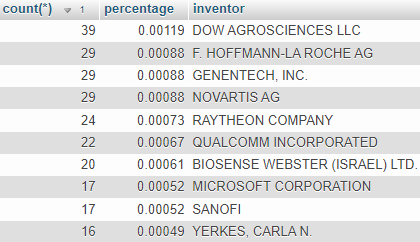
\includegraphics[width=9cm]{img/scenare/scenar_1}
\caption{Ukázka výsledku dotazu pro scénář č.1}
\label{fig:scenar1}
\end{figure}

\newpage
\subsection{Scénář č.2}
\textbf{Textový popis}: Pět nejméně patentovaných oborů v Kanadě od roku 2010.
\newline
\textbf{Název pohledu}: five\_CA\_sections\_ge\_2010
\newline
\textbf{SQL}: 
\begin{lstlisting}[label = {lst:elements_a}]
select count(*), count(*) * 100.0 / ((select count(*) from patent_classification left outer join patents on patents.id = patent_classification.id_patent where YEAR(patents.patent_date) >= 2010 and patents.patent_id like '%CA%') * 1.0) as percentage, classification.section from classification left outer join patent_classification on classification.id = patent_classification.id_classification left outer join patents on patents.id = patent_classification.id_patent where YEAR(patents.patent_date) >= 2010 and patents.patent_id like '%CA%' group by classification.section order by count(*) asc, percentage asc LIMIT 5;
\end{lstlisting}
\textbf{Rychlost vykonání dotazu}: \textpm 10 sekund
\newline
\textbf{Výsledek dotazu}: Na obrázku č. \ref{fig:scenar2} lze vidět výsledek scénáře. Mezi nejméně patentované obory v Kanadě se nachází \textit{textílie} (D), \textit{pevné konstrukce} (E), \textit{strojírenství} (F), \textit{elektřina} (H) a \textit{fyzika} (G).
\begin{figure}[H]
\centering
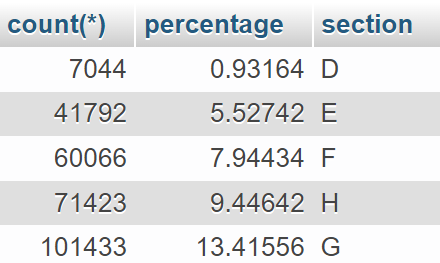
\includegraphics[width=5cm]{img/scenare/scenar_2}
\caption{Ukázka výsledku dotazu pro scénář č.2}
\label{fig:scenar2}
\end{figure}

\newpage
\subsection{Scénář č.3}
\textbf{Textový popis}: Dvacet nejčastějších klasifikací patentů za rok 2008 ve Španělsku.
\newline
\textbf{Název pohledu}: twenty\_ES\_classification\_2008
\newline
\textbf{SQL}:
\begin{lstlisting}[label = {lst:elements_a}]
select count(*), count(*) * 100.0 / ((select count(*) from patent_classification left outer join patents on patents.id = patent_classification.id_patent where YEAR(patents.patent_date) = 2008 and patents.patent_id LIKE '%ES%') * 1.0) as percentage, classification.section, classification.class, classification.subclass from classification left outer join patent_classification on classification.id = patent_classification.id_classification left outer join patents on patents.id = patent_classification.id_patent where YEAR(patents.patent_date) = 2008 and patents.patent_id LIKE '%ES%' group by classification.section, classification.class, classification.subclass order by count(*) desc, percentage desc LIMIT 20;
\end{lstlisting}
\textbf{Rychlost vykonání dotazu}: \textpm 1,3 sekundy
\newline
\textbf{Výsledek dotazu}: Na obrázku č. \ref{fig:scenar3} lze vidět výsledek scénáře. Nejčastější klasifikace patentů je: \textit{kontejnery pro skladování nebo přepravu předmětů nebo materiálů} (B65D). Většina patentů spadá pod obory \textit{pevné konstrukce} (E) a \textit{lidské potřeby} (A).
\begin{figure}[H]
\centering
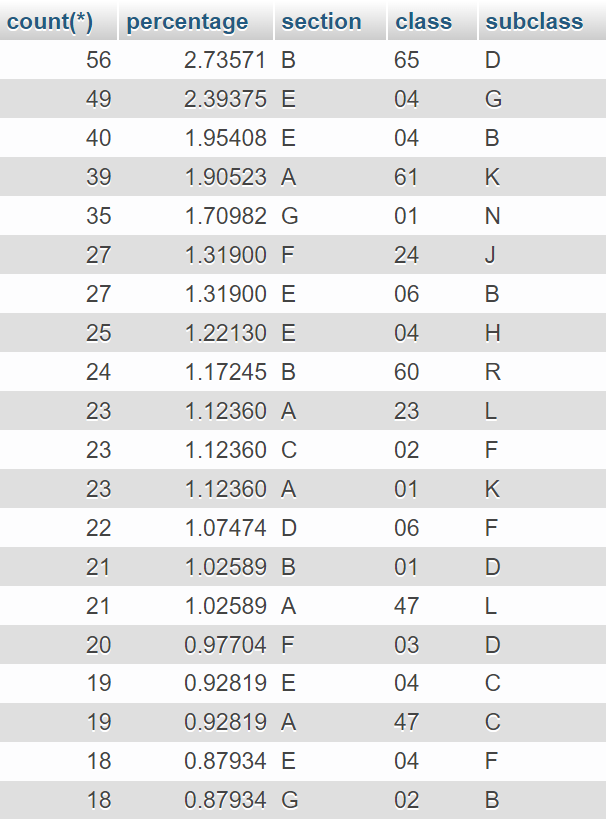
\includegraphics[width=7cm]{img/scenare/scenar_3}
\caption{Ukázka výsledku dotazu pro scénář č.3}
\label{fig:scenar3}
\end{figure}

\newpage
\subsection{Scénář č.4} 
\textbf{Textový popis}: Deset autorů / institucí s největším počtem patentů ze všech zemí.
\newline
\textbf{Název pohledu}: ten\_most\_authors
\newline
\textbf{SQL}: 
\begin{lstlisting}[label = {lst:elements_a}]
select count(*), count(*) * 100.0 / ((select count(*) from inventors) * 1.0) as percentage, inventors.inventor from inventors group by inventors.inventor order by count(*) desc, percentage desc LIMIT 10;
\end{lstlisting}
\textbf{Rychlost vykonání dotazu}: \textpm 1,5 sekundy
\newline
\textbf{Výsledek dotazu}: Na obrázku č. \ref{fig:scenar4} lze vidět výsledek scénáře. Z výsledků vyplývá, že nejvíce aktivních autorů / institucí je z ruska (celkem čtyři z~deseti). 
\begin{figure}[H]
\centering
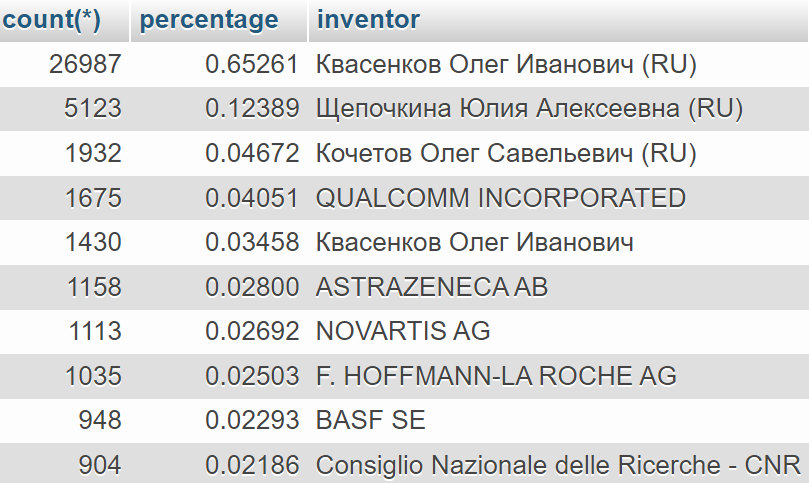
\includegraphics[width=8cm]{img/scenare/scenar_4}
\caption{Ukázka výsledku dotazu pro scénář č.4}
\label{fig:scenar4}
\end{figure}

\newpage
\subsection{Scénář č.5}
\textbf{Textový popis}: Pět nejméně používaných jazyků pro patenty za rok 2003.
\newline
\textbf{Název pohledu}: five\_languages\_2003
\newline
\textbf{SQL}: 
\begin{lstlisting}[label = {lst:elements_a}]
select count(*), count(*) * 100.0 / ((select count(*) from patents where patents.language not like '%-%') * 1.0) as percentage, patents.language from patents where patents.language not like '%-%' group by patents.language order by count(*) asc, percentage asc LIMIT 5;
\end{lstlisting}
\textbf{Rychlost vykonání dotazu}: \textpm 3,3 sekundy
\newline
\textbf{Výsledek dotazu}: Na obrázku č. \ref{fig:scenar5} lze vidět výsledek scénáře. Z výsledků vyplývá, že nejméně používaný jazyk u patentů je \textit{Portugalština}, \textit{Litevština} a \textit{Španělština}. \textit{Francouzština} a \textit{Ruština} mají už celkem velké procento zastoupení.
\begin{figure}[H]
\centering
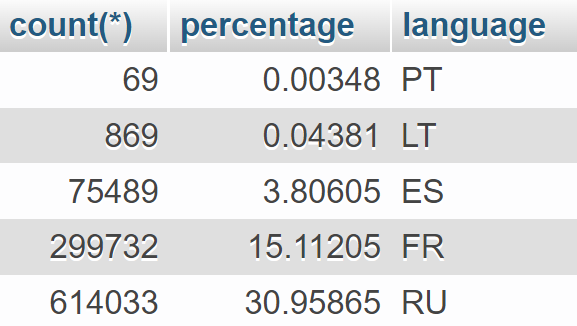
\includegraphics[width=5cm]{img/scenare/scenar_5}
\caption{Ukázka výsledku dotazu pro scénář č.5}
\label{fig:scenar5}
\end{figure}

\newpage
\subsection{Scénář č.6}
\textbf{Textový popis}: Deset Institucí / autorů s patenty pokrývající největší množství oborů ve Španělsku.
\newline
\textbf{Název pohledu}: ten\_ES\_authors\_most\_kinds
\newline
\textbf{SQL}: 
\begin{lstlisting}[label = {lst:elements_a}]
select count(distinct classification.section), count(*) * 100.0 / ((select count(*) from inventors left outer join patents on patents.id = inventors.id_patent left outer join patent_classification on patents.id = patent_classification.id_patent left outer join classification on classification.id = patent_classification.id_classification where classification.section is not null and patents.country like '%ES%') * 1.0) as percentage, inventors.inventor from inventors left outer join patents on patents.id = inventors.id_patent left outer join patent_classification on patents.id = patent_classification.id_patent left outer join classification on classification.id = patent_classification.id_classification where classification.section is not null and patents.country like '%ES%' group by inventors.inventor order by count(distinct classification.section) desc, percentage desc LIMIT 10;
\end{lstlisting}
\textbf{Rychlost vykonání dotazu}: \textpm 1,8 sekundy
\newline
\textbf{Výsledek dotazu}: Na obrázku č. \ref{fig:scenar6} lze vidět výsledek scénáře. Na prvním a druhém místě si lze povšimnout, že jméno vynálezce je totožné, pouze jinak zapsané.
\begin{figure}[H]
\centering
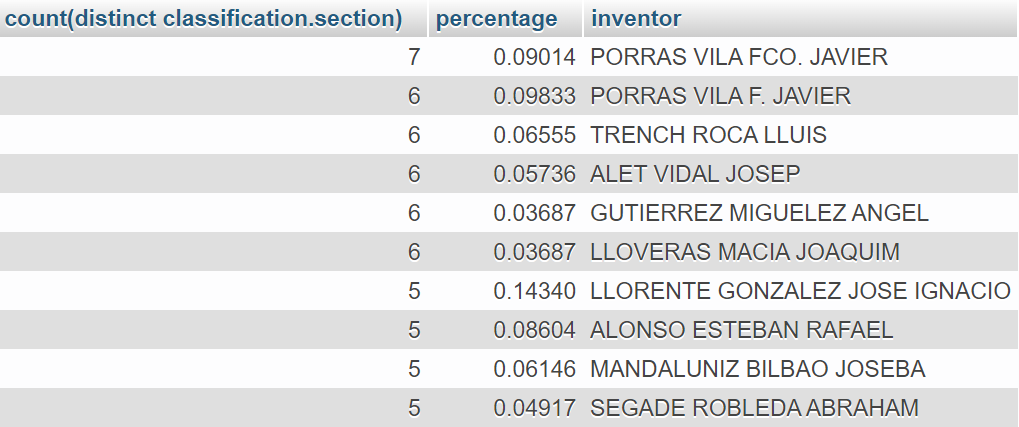
\includegraphics[width=10cm]{img/scenare/scenar_6}
\caption{Ukázka výsledku dotazu pro scénář č.6}
\label{fig:scenar6}
\end{figure}

\newpage
\subsection{Scénář č.7}
\textbf{Textový popis}: Pět zemí s nejvíce patenty od roku 2018.
\newline
\textbf{Název pohledu}: five\_most\_country\_ge\_2018
\newline
\textbf{SQL}: 
\begin{lstlisting}[label = {lst:elements_a}]
select count(*), count(*) * 100.0 / ((select count(*) from patents where YEAR(patents.patent_date) >= 2018) * 1.0) as percentage, patents.country from patents where YEAR(patents.patent_date) >= 2018 group by patents.country order by count(*) desc, percentage desc LIMIT 5;
\end{lstlisting}
\textbf{Rychlost vykonání dotazu}: \textpm 1,3 sekundy
\newline
\textbf{Výsledek dotazu}: Na obrázku č. \ref{fig:scenar7} lze vidět výsledek scénáře. Mezi nejčastěji patentující země od roku 2018 lze zařadit hlavně \textit{Rusko}, \textit{Kanadu} a \textit{Francii}, které dohromady pokrývají přibližně 94\% všech patentů.
\begin{figure}[H]
\centering
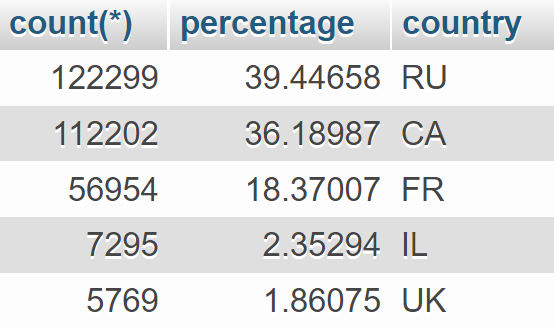
\includegraphics[width=5cm]{img/scenare/scenar_7}
\caption{Ukázka výsledku dotazu pro scénář č.7}
\label{fig:scenar7}
\end{figure}

\newpage
\subsection{Scénář č.8}
\textbf{Textový popis}: Nejvíce používaný typ patentu ve Francii.
\newline
\textbf{Název pohledu}: most\_FR\_kind
\newline
\textbf{SQL}: 
\begin{lstlisting}[label = {lst:elements_a}]
select count(*), count(*) * 100.0 / ((select count(*) from patents where patents.patent_id like '%FR%' and patents.kind not like '%-%') * 1.0) as percentage, patents.kind from patents where patents.patent_id like '%FR%' and patents.kind not like '%-%' group by patents.kind order by count(*) desc, percentage desc;
\end{lstlisting}
\textbf{Rychlost vykonání dotazu}: \textpm 3,1 sekundy
\newline
\textbf{Výsledek dotazu}: Na obrázku č. \ref{fig:scenar8} lze vidět výsledek scénáře. Přibližně 98\% všechn patentů ve Francii má typ: \textit{patent na vynález}.
\begin{figure}[H]
\centering
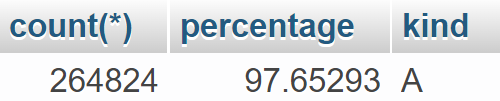
\includegraphics[width=5cm]{img/scenare/scenar_8}
\caption{Ukázka výsledku dotazu pro scénář č.8}
\label{fig:scenar8}
\end{figure}

\newpage
\subsection{Scénář č.9}
\textbf{Textový popis}: Patnáct nejčastěji patentujících institucí / autorů ve Velké Británii v textilním oboru za rok 2013.
\newline
\textbf{Název pohledu}: fifteen\_UK\_author\_textile\_2013
\newline
\textbf{SQL}: 
\begin{lstlisting}[label = {lst:elements_a}]
select count(*), count(*) * 100.0 / ((select count(*) from inventors left outer join patents on patents.id = inventors.id_patent left outer join patent_classification on patents.id = patent_classification.id_patent left outer join classification on classification.id = patent_classification.id_classification where classification.section like '%D%' and patents.patent_id like '%GB%' and YEAR(patents.patent_date) = 2013) * 1.0) as percentage, inventors.inventor from inventors left outer join patents on patents.id = inventors.id_patent left outer join patent_classification on patents.id = patent_classification.id_patent left outer join classification on classification.id = patent_classification.id_classification where classification.section like '%D%' and patents.patent_id like '%GB%' and YEAR(patents.patent_date) = 2013 group by inventors.inventor order by count(*) desc, percentage desc LIMIT 15;
\end{lstlisting}
\textbf{Rychlost vykonání dotazu}: \textpm 0,3 sekundy
\newline
\textbf{Výsledek dotazu}: Na obrázku č. \ref{fig:scenar9} lze vidět výsledek scénáře. Ve Velké Británii v roce 2013 patentují vynálezy v textilním oboru hlavně lidé (ne instituce a firmy, ty mohou být registrováni například jako žadatelé). 
\begin{figure}[H]
\centering
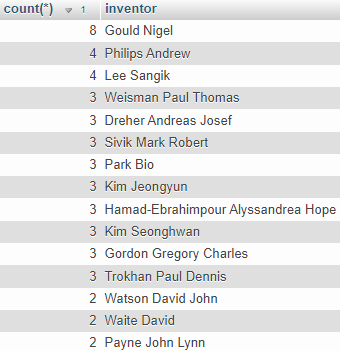
\includegraphics[width=9cm]{img/scenare/scenar_9}
\caption{Ukázka výsledku dotazu pro scénář č.9}
\label{fig:scenar9}
\end{figure}